\subsection{Phân tích lỗi và trực quan hóa kết quả}
\label{sec:erroranalysis}
\begingroup
\setlength{\intextsep}{6pt}
Trên 438 câu dev có 593 cặp câu hỏi--điều luật theo gold; hệ thống trả đúng 387 cặp và bỏ sót 206 cặp. Hình~\ref{fig:errorcounts} phân các cặp bị bỏ sót thành ba nhóm không chồng lấn: không vào tập ứng viên, có trong tập nhưng ngoài top-5 sau LightGBM, hoặc nằm trong top-5 nhưng bị điểm cắt loại.
\begin{figure}[H]
\centering
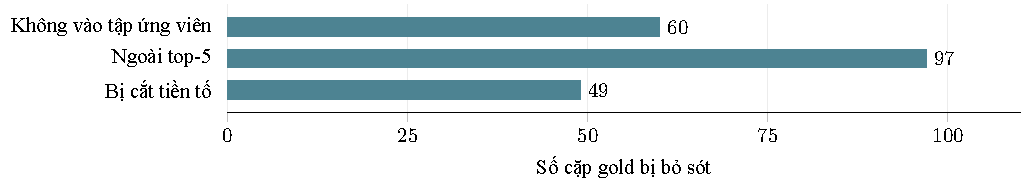
\includegraphics[width=.95\textwidth]{figures/error_counts.pdf}
\caption{Phân bố các cặp gold bị bỏ sót; top-5 xét sau LightGBM, trước chọn tiền tố.}
\label{fig:errorcounts}
\end{figure}
Các số đếm được cộng theo cặp; Recall ở Bảng~\ref{tab:policies} lấy trung bình theo câu hỏi. Nhóm ngoài top-5 chiếm nhiều nhất (97/206), gợi ý cần cải thiện thứ hạng bên cạnh chọn độ dài. Bảng~\ref{tab:errorcases} minh họa hai lỗi ở bước chọn kết quả: cắt thiếu một gold đã xếp cao và giữ thêm ứng viên cùng chủ đề nhưng ngoài nhãn.
\begin{table}[H]
\centering\small
\caption{Hai trường hợp minh họa lỗi chọn số điều luật trên tập dev.}
\label{tab:errorcases}
\renewcommand{\arraystretch}{1.12}
\begin{tabularx}{\textwidth}{@{}>{\raggedright\arraybackslash}p{4.1cm}>{\raggedright\arraybackslash}p{1.65cm}>{\raggedright\arraybackslash}p{1.65cm}Y@{}}
\toprule
Câu hỏi (qid) & Gold (aid) & Trả về (aid) & Nhận xét\\
\midrule
14663: Vi bằng phải đảm bảo nội dung và hình thức thế nào? & 29868, 29872 & 29872 & Giữ top-1 dù hai gold ở hạng 1--2 sau LightGBM; mã 29868 bị bỏ tại điểm cắt.\\
2406: Người khuyết tật được ưu tiên mua vé xe buýt không? & 19739 & 19739, 57446 & Mã 57446 nói về miễn, giảm giá vé; gần chủ đề nhưng ngoài gold của câu hỏi về ưu tiên mua vé.\\
\bottomrule
\end{tabularx}
\end{table}
\endgroup
